\documentclass[a4paper,12pt]{article}
\linespread{1.5}
\usepackage[left=2cm,top=2cm,right=2cm,bottom=2cm]{geometry}

%\usepackage{palatino}

\usepackage{xypic}
\usepackage{natbib}
\bibliographystyle{plainnat}
\bibpunct{[}{]}{;}{s}{,}{,}

\usepackage[header,page,titletoc]{appendix}
\renewcommand{\appendixname}{Appendix}
%\renewcommand{\appendixtocname}{List of appendices}

\usepackage[colorlinks=true,linkcolor=black,citecolor=black,filecolor=black,menucolor=black,urlcolor=black]{hyperref}
\usepackage{graphicx}
\usepackage{amsmath}
\usepackage{pdfpages}
\usepackage{wrapfig}
\usepackage{fancyhdr}
\usepackage{pict2e}
\setlength{\headheight}{15.2pt}

\pagestyle{fancy}
\usepackage{cite}
%
% fix citations to be IEEE style
\def\citepunct{], [}
\def\citedash{]--[}

\newcommand{\nonumsection}[1]{
\section{#1}
%\addcontentsline{toc}{section}{#1}
}


\newenvironment{packed_itemize}{
\begin{itemize}
  \setlength{\itemsep}{1pt}
  \setlength{\parskip}{0pt}
  \setlength{\parsep}{0pt}
}{\end{itemize}}

%Used to change "Abstract" to "Executive Summary"

% Paragraph Settings
\setlength{\parindent}{0pt}
\setlength{\parskip}{5pt}

\begin{document}
\thispagestyle{empty}
\vspace*{\fill}
\includegraphics[width=10cm]{./UofAlogo2.pdf}\\
\noindent
\textsc{
\textsc{School of Electrical \& Electronic Engineering}\\
Adelaide, South Australia, 5005\\ \\
}
\noindent
\Large{\textbf{
ELEC ENG 4039A/B \\
Honours Project\\
	}}
	\Large{
		A Radio Relay System for Remote Sensors in the Antarctic \\
	}
	\small{\textbf{Supervisor: Assoc. Prof. Chris Coleman}}\\
	\small{\textbf{Moderator: Dr. Christophe Fumeaux}}
	\ \\
	\ \\
	\Large{\textbf{
		Final Report \\
	}}
	\ \\
	\small{\textbf{
		Written by: \\}
		Mark Jessop \\
		1163807
	}
	\ \\
	\ \\
	Date Submitted: October 25, 2010 \\
	Signature of Supervisor: \\
 %\end{center}
 \vspace*{\fill}

\newpage
 \thispagestyle{empty}
 \vspace*{\fill}
\begin{abstract}
\noindent
A common problem with remote sensor systems is the retrieval of data. Satellite-based systems are expensive, as is travelling to the sensor. HF propagation provides an inexpensive alternative. Radio signals below 30MHz bounce off the ionosphere, travelling thousands of kilometres using only a few watts of transmit power.
Based around an Atmel XMega Micro-Controller and using Direct Digital Synthesis techniques, this project aims to provide a reliable low power HF telemetry system, usable in a variety of remote telemetry applications. 
By making use of the XMega's power-save modes and using high-efficiency RF amplifiers, power consumption is minimised, allowing months of operation from battery power.
\end{abstract}
\vspace*{\fill}
\newpage
\setcounter{tocdepth}{2}
\tableofcontents
\newpage

\section{Introduction}
Many scientific experiments require data logging over a long time period, and in remote locations. To further research progress, it is desirable for the collected data to be accessible throughout the run of the experiment.

A number of solutions exist to obtain data from a remote sensor unit. The first is to physically access the remote sensor station, and copy data from whatever storage may exist. For very remote sensor units visiting the site may be impractical or too costly, so some form of wireless communication is often used. 

Satellite data transmission is a reliable way of retrieving data, but comes at a high cost. For example, using the Iridium Satellite constellation to transmit data would cost approximately USD\$2.50 per minute, with a 2400 baud data rate\citep{ref:iridium}.

The other option is to other methods of radio communication. For reasonably short ($<$50km) distances VHF (30-300MHz) or UHF (300-3000MHz) telemetry can be used. For example, the Australian Bureau of Meteorology uses a network of VHF transmitters\citep{ref:bomtx} and repeaters to obtain data from weather stations around Adelaide. VHF and UHF can work for longer distances ($>$50km), but with less reliability. VHF and UHF operation at these distances relies on tropospheric ducting, a phenomenon based on atmospheric temperature inversion that is not always present. To obtain high reliability long distance transmission, we must move further down the electromagnetic spectrum, to the HF (`high frequency') band.

\subsubsection*{The Ionosphere}

Radio waves in the HF band propagate by two means: ground-wave and sky-wave. Ground-wave, as the name suggests, travel along the surface of the earth. Ground-wave signals are attenuated as they travel along the earth's surface, limiting their distance. Sky-waves however, refract off a charged region of the earth's atmosphere called the ionosphere, and can travel many thousands of kilometers.

\begin{figure}[h]
  \begin{center}
    \includegraphics[width=0.6\textwidth]{images/ionosphere.png}
  \end{center}
  \caption{Ionospheric Layers}
  \label{fig:ionosphere}
\end{figure}

The ionosphere is made up of a number of complex and ever-changing layers of ionised particles that surround our planet. The different layers are given the letters D, E and F. The D-layer, which is the lowest and is strongest during the day, absorbs RF energy below a certain frequency. The E and F layers, however, \textit{reflect} RF energy below a certain \textit{critical frequency}, $f_c$. This property enables HF radio signals to be `bounced' off the ionosphere, even multiple times, to communicate over long distances. Losses from the D-layer, and the critical frequencies of the E and F layers determine the Lowest Usable Frequency (LUF) and Maximum Usable Frequency (MUF) for long distance communication. Ionospheric prediction services, such as the one provided by the Australian government \citep{ref:bom}, provide tools to predict these frequencies and hence determine the optimal frequency for reliable communication.

Another consideration is the angle at which a radio wave interacts with the ionosphere. If a radio signal is aimed at the horizon it will hit the ionosphere at a shallow angle, resulting in very long propagation distances, potentually thousands of kilometres. For shorter distances the signal is aimed close to vertical, allowing much shorter hops of a few hundred kilometres. This method of transmission is called `Near Vertical-Incidence Skywave' (NVIS) and is the primary method this project will use to transmit data.

\subsubsection*{Project Applications \& Aim}

\begin{quote}
\textit{
Design and build a low power short wave data transmitter that can translate low rate data into a modulated short wave output with sufficient power to transmit the data over several hundred kilometres on an Antarctic communication path.}
- Original Project Aim
\end{quote}

\begin{figure}[h]
  \begin{center}
    \includegraphics[width=0.9\textwidth]{images/Antarctic_Radio_Overview.pdf}
  \end{center}
  \caption{High-Level Overview of Transmitter}
  \label{fig:high_level}
\end{figure}

At its core, the purpose of the transmitter is to read in data from a number of sources, buffer the data, and then transmit it using HF radio modulation. This is accomplished using a transmission system consisting of a core micro-controller, a signal generator, and an amplifier (Figure \ref{fig:high_level}).

Having a `smart' CPU in the system, as opposed to some kind of `dumb' transmitter, means the opportunity exists to build in some more advanced features. For example, if the data being collected related to the state of the ionosphere, the data itself could be used to determine the optimal data transmission frequency. Alternatively, a small receiver could be attached to receive commands from home base, and change operational parameters.

Originally intended to be used by a researcher in Antarctica, the project's scope was expanded to include other telemetry applications. The British Antarctic Survey have expressed interest in operating this system on remote islands in the south atlantic ocean. Closer to home, a local high-altitude ballooning group offered to launch a prototype transmitter to test it's usefulness as an in-flight telemetry system.


The exact form of HF modulation was not defined, to allow experimentation with a number of different modes. To enable high power testing without licensing issues, it was decided that the 80m (3.5MHz) and 40m (7MHz) amateur radio bands would be used. This also had the added benefit of having a large number of radio operators available to report on signal reception.

To keep the spirit of the original application it was decided to keep the constraints which Antarctic operation required. These were:
\begin{enumerate}
\item Operation at extremely cold temperatures ($<-30^\circ$C), such as those commonly experienced in Antarctica.
\item High energy efficiency to enable operation from battery power for long periods of time, possibly months.
\end{enumerate}

Testing these constraints proved straightforward. Testing the actual operation of the transmitter proved harder. To check if the output signal was propagating via skywave, help was enlisted from various amateur operators, who could provide reception reports. 

To provide an overall test of how the hardware would operate in harsh conditions, a prototype was constructed and launched beneath a high altitude weather balloon to 32km above sea level. This subjected the prototype to the extreme ($-40^\circ$C) temperatures of the upper atmosphere, in which it performed perfectly.


\newpage
\section{Hardware}

\subsection{CPU}
\begin{wrapfigure}{r}{0.3\textwidth}
  \begin{center}
    \includegraphics[width=0.28\textwidth]{images/xmega100.jpg}
  \end{center}
  \caption{XMega100 Breakout Board}
  \label{fig:xmega100}
\end{wrapfigure}
The main CPU of the HF transmitter is an Atmel AT-XMega128A1, an 8-bit micro-controller running at clock speeds up to 32MHz. It has numerous peripherals, such as 12-bit ADCs (Analog to Digital Converters), a 12-bit DAC (Digital to Analog Converter), and 64 I/O (Input/Output) lines\citep{ref:xmega}. A particularly useful feature is the ability to wire SD-RAM into three of the I/O ports and have the extra memory appear at the end of the XMega's memory space. This is called the `External Bus Interface' (EBI) and allows the buffering of large portions of data with little external circuitry.

The XMega was chosen over other similar micro-controllers (such as the Texas Instruments MSP430) primarily due to the open-source and cross-platform compiler tools available. Software development was primarily carried out on an Apple Macbook, and having a compiler and programmer working without rebooting into Microsoft Windows proved very useful.

\begin{wrapfigure}{l}{0.4\textwidth}
  \begin{center}
    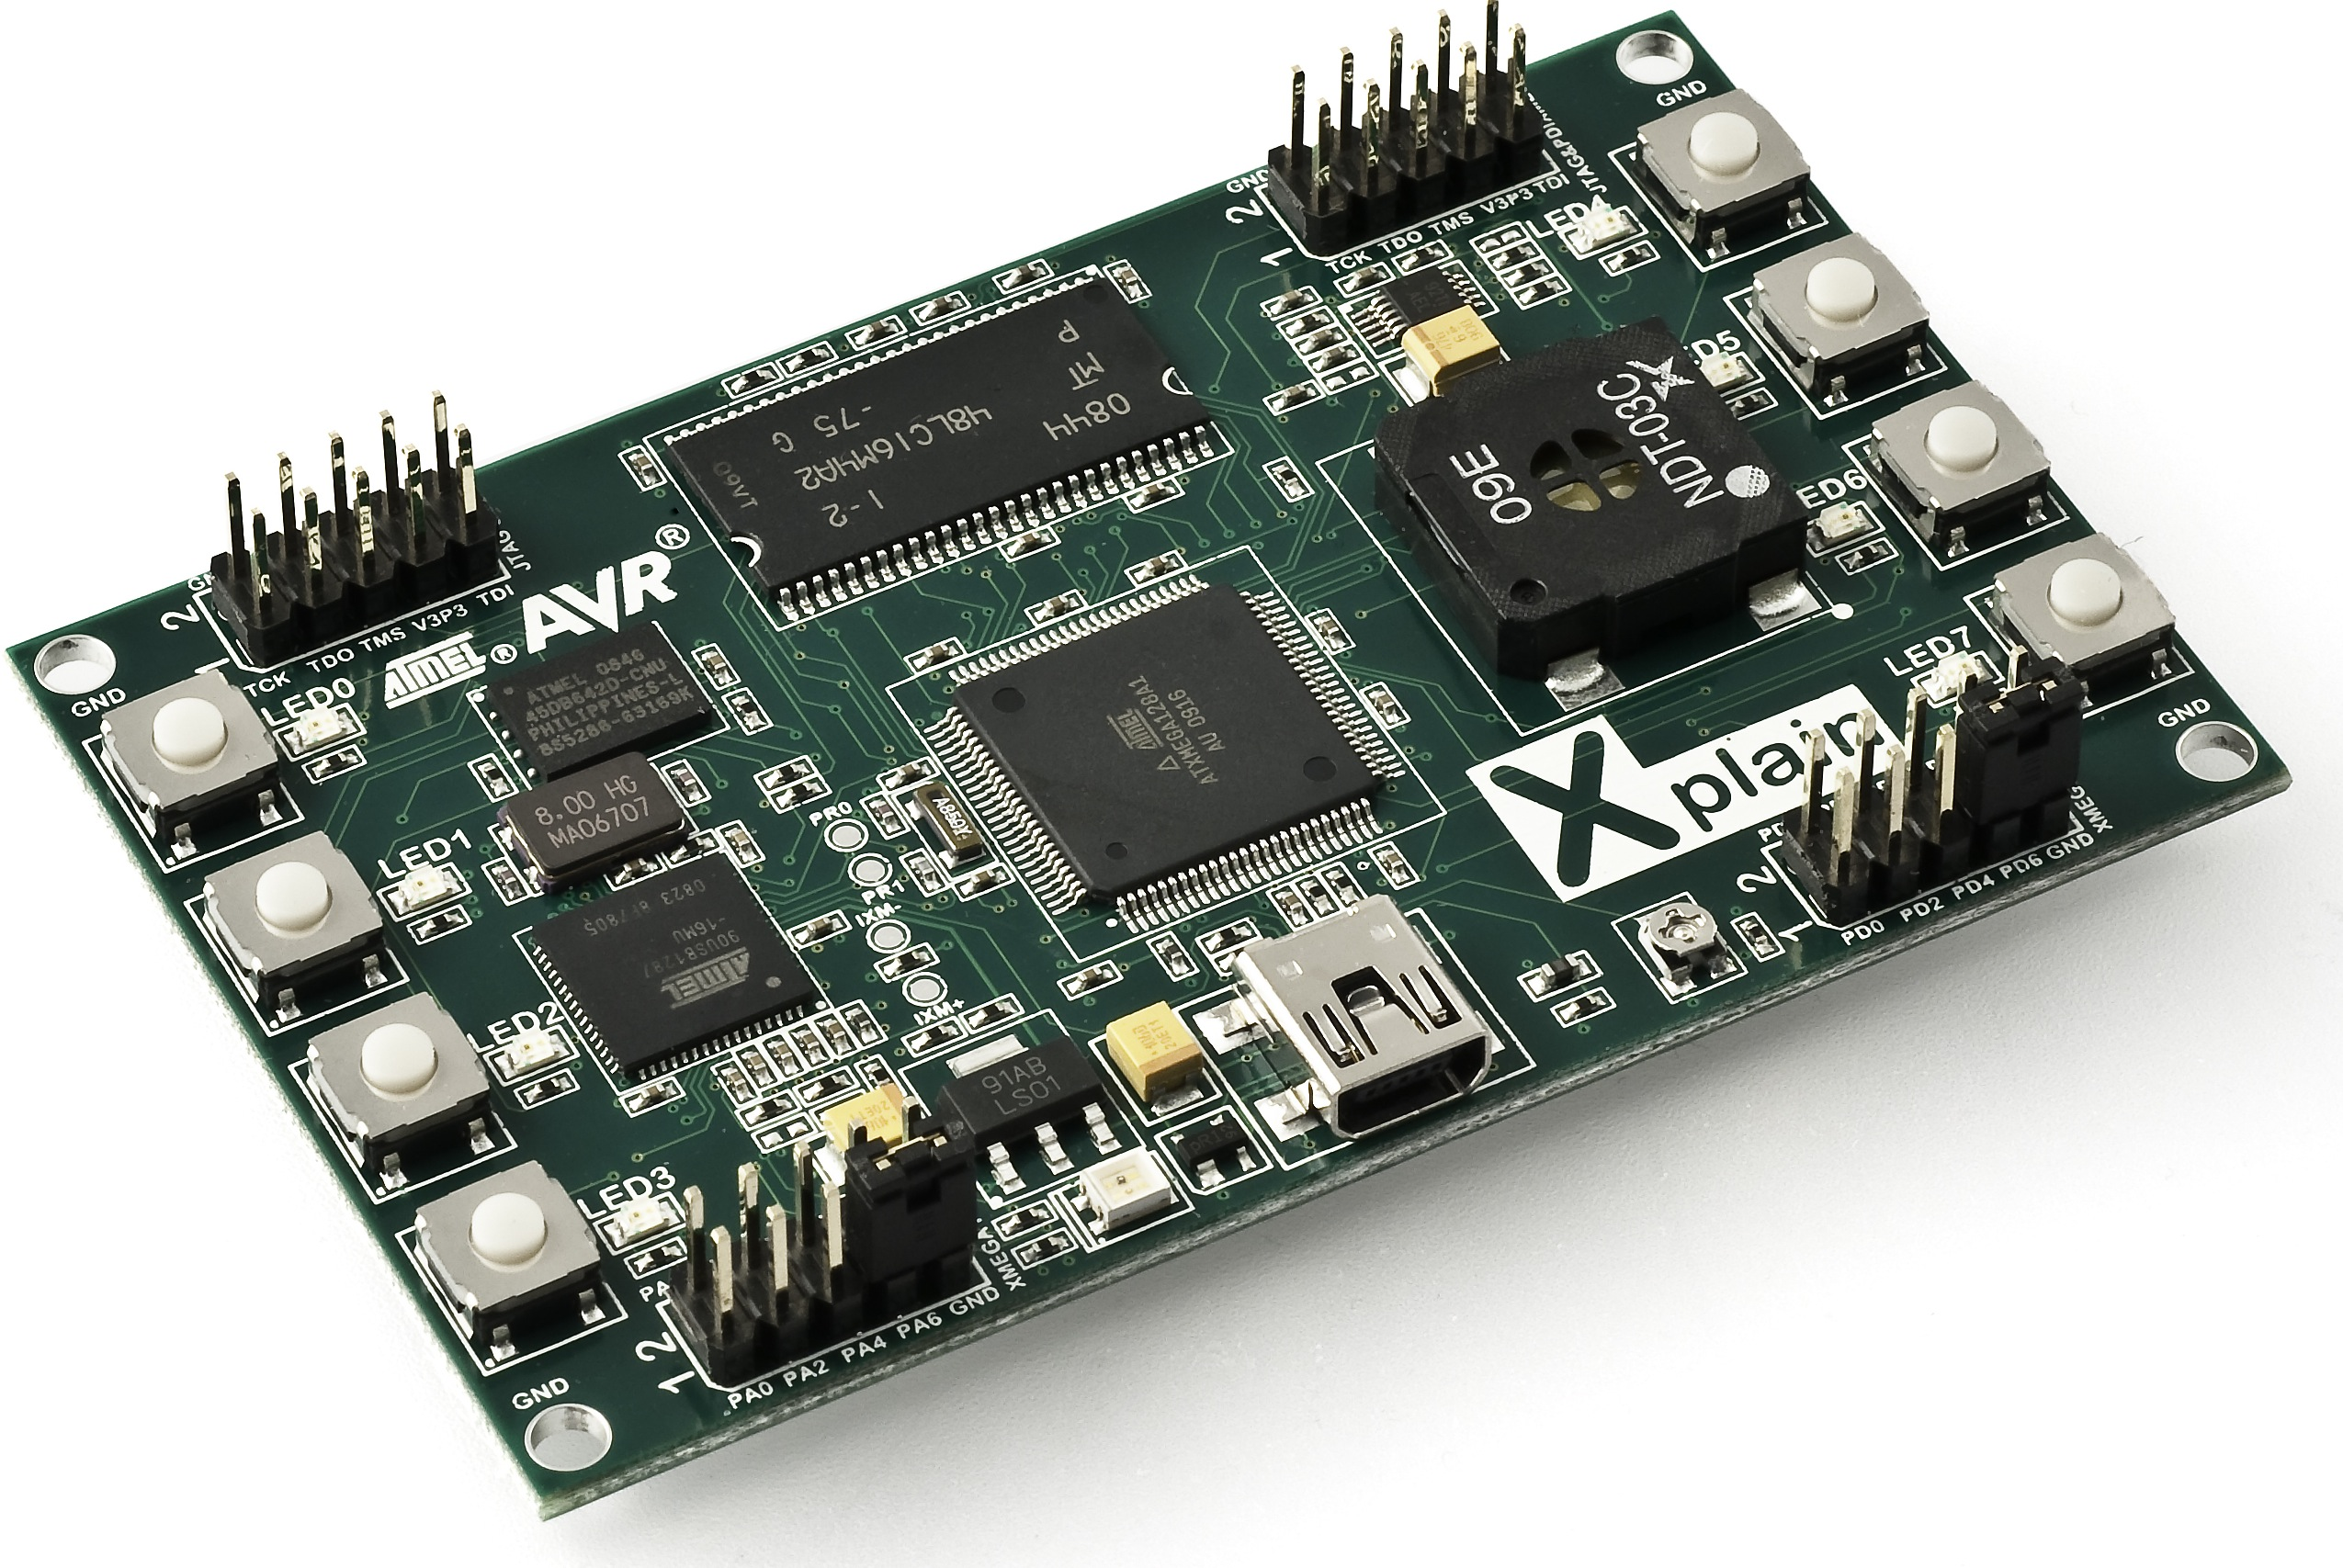
\includegraphics[width=0.4\textwidth]{images/xplain.jpg}
  \end{center}
  \caption{XPlain Development Board}
  \label{fig:xplain}
\end{wrapfigure}

For the purposes of easy development, two breakout boards were purchased. The first, a Sparkfun XMega100 breakout board (Figure \ref{fig:xmega100}), simply gives access to the I/O pins on the IC, and was bought as a means to evaluate the micro-controller as a viable platform. The second, an Atmel XPlain development board, has buttons, LEDs, and a number of extra peripherals, such as 8MB of SDRAM and 8MB of NAND-Flash memory. This board was used for most development work, as the buttons and LEDs proved extremely useful for debugging code. One downside of the XPlain board is that all the extra ICs cannot be disabled, resulting in the entire board drawing about 100mA @ 3.3V, depending on how many LEDs are illuminated.

When running at 32MHz with most peripherals disabled, the XMega was measured to draw 20mA of current at 3.3V. Running at 2MHz, the current draw was measured at 2mA. The XMega also has a number of power-save modes, where an ultra-low-power 32KHz oscillator is used. The XMega's data-sheet states these modes draw between 0.1 and $3\mu A$ depending on what functions are enabled, but this has not been tested. From this information we can see that the XMega's power requirements are extremely minimal, especially when running at low clock speeds.

To see if the XMega128A1 would satisfy the cold-climate operation requirement, the Sparkfun breakout board was subjected to low temperature testing. Using frozen CO$_2$ (dry-ice), the temperature of the XMega was lowered to $-54^\circ$C. The internal 32MHz oscillator drifted upwards to 33MHz, with the XMega still continuing to function. Further details of the test process appear in  Appendix \ref{xmegadryice}.


\subsection{Signal Generator}
\begin{wrapfigure}{r}{0.3\textwidth}
  \begin{center}
    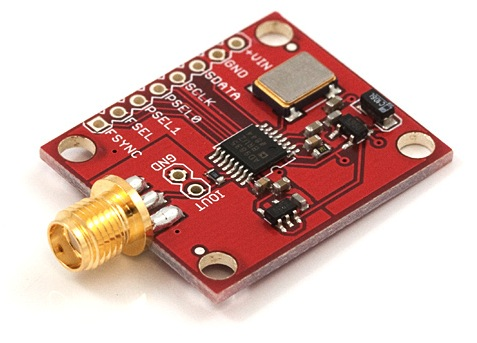
\includegraphics[width=0.28\textwidth]{images/ad9835.jpg}
  \end{center}
  \caption{AD9835 Breakout}
  \label{fig:ad9835}
\end{wrapfigure}
The start of the transmitter's RF section begins with the signal generator. Two signal generators were experimented with for this project, the Analog Devices AD9834 and AD9835. Both devices are programmable Direct Digital Synthesis (DDS) signal generators, able to produce sine wave output between 1Hz and 25MHz. The output amplitude varies depending on frequency - a plot showing this can be seen in Figure \ref{fig:ad9835_output}.

\begin{figure}%[h]
  \begin{center}
    \includegraphics[width=0.7\textwidth]{images/AD9835_Output.pdf}
  \end{center}
  \caption{AD9835 Frequency Response}
  \label{fig:ad9835_output}
\end{figure}

Inside each device is a 10-bit 50Msps (Mega-samples per second) DAC, clocked using an external 50MHz oscillator. Serial Peripheral Interface (SPI) programmed control registers allow the programming of two different frequencies. These can be selected between using either control bits or a dedicated input pin, allowing FSK modulation. The registers can be reprogrammed approximately 7500 times per second, allowing MFSK modulation with high symbol rates. Phase registers (2 in the AD9834, 4 in the AD9835) permit BPSK and QPSK modulation, though this was not used in the project.

The AD9834 is a lower power device, drawing 8mA at 5V, while the AD9835 can draw up to 40mA. In practice, it was found that when the current draw of the required master oscillator was included, the power requirements of both devices (with supporting circuitry) were very similar (~35mA @ 5V).

The AD9835 was purchased on a breakout board from Sparkfun prior to the project, which started the idea of using a DDS to power the RF section. The AD9834 was purchased as a bare IC, and a breakout PCB was designed and constructed for it. Schematics and PCB designs for this board appear in Appendix \ref{ad9834_breakout}. The breakout was originally designed to run at 3.3V, the same voltage level as the micro-controller. However, because the board ended up using a 5V master oscillator (3.3V models were not available at the time), it had to be operated entirely at 5V. Even running at 5V the AD9834 accepts 3.3v logic levels from the XMega, unlike the 5V AD9835 which requires logic level conversion.

Being a DAC-based signal generator, the output waveform is not a pure sine. Sampling theory tells us that at 10MHz we would only 5 samples per cycle, and at 25MHz only 2 samples per cycle. At the target frequency of 7MHz, clock feedthrough (50MHz) was measured at -20dB below the target output. In Australia, spurious emissions should be -30dB below the fundamental frequency, so a reasonably sharp low-pass filter was designed to drop the clock feedthrough down by about -50dB. Use of a tuned antenna will may also attenuate the clock feedthrough enough to meet legal limits, but this could not be tested easily.

Another concern with any signal generator is how the output frequency drifts with temperature. To test this, the AD9835 was programmed to output a 7MHz sine, and was then placed in dry-ice. Over the course of an hour, the temperature of the AD9835 dropped to $-40^\circ$C, with the output frequency drifting upwards by 300Hz. This amount of drift is easily compensated for on the receiving end, and is of no concern to this project.

\begin{figure}[h]
  \begin{center}
    \includegraphics[width=0.8\textwidth]{images/ad9835_drift.pdf}
  \end{center}
  \caption{AD9835 Frequency Drift}
  \label{fig:ad9835_drift}
\end{figure}

Figure \ref{fig:ad9835_drift} shows a spectrogram of the output from a Yaesu FRG-8800 receiver as the AD9835 was cooled. Note that the frequency scale shows the demodulated frequency, with the receiver not being accurately tuned. 

\subsection{Low Pass Filter}
\begin{figure}
  \begin{center}
    \includegraphics[width=0.4\textwidth]{images/AD9835_LPF_Schem.pdf}
  \end{center}
  \caption{AD9835 LPF Schematic}
  \label{fig:ad9835_lpf_schem}
\end{figure}

\begin{figure}
  \begin{center}
    \includegraphics[width=0.7\textwidth]{images/AD9835_LPF.pdf}
  \end{center}
  \caption{AD9835 LPF Frequency Response}
  \label{fig:ad9835_lpf}
\end{figure}

A low pass filter was built using a design with a cutoff frequency of about 11MHz, using a design from a similar DDS project\citep{ref:lpf}.  

The filter is composed of a 5th order low-pass filter combined with two notch filters. The rolloff is very sharp, dropping to -150dB within 8MHz, before rising again to -50dB at 40MHz. This filter has -15dB of insertion loss at 7MHz, but this can be compensated for using the following pre-amplifier. This filter design proved useful later in the project, as it heavily attenuates the 2nd harmonic when operating with a 7MHz carrier.

\subsection{Pre-Amplifier}

As the output from the AD9835 (and the filter) has too little power to drive a high powered amplifier, a pre-amp needed to be built. To enable flat gain over the signal generator's wide bandwidth, an op-amp based amplifier was designed and constructed. The amplifier is based around a wide-bandwidth Analog Devices AD8008 dual op-amp IC, running from a 12V supply. Schematics of the amplifier, and a PCB design, appear in Appendix \ref{ad8008_preamp}.

\subsubsection*{Operation}

The amplifier uses both op-amps in series, in a non-inverting configuration. The second op-amp is set to have a gain of 6dB, while the first has a gain variable between 4.7dB and 13dB, giving a total gain between 10.9dB and 19dB. The input signal is biased to half the supply voltage, to attempt to stop the signal hitting the supply or ground rails. Input and output impedances of the amplifier are both approximately $50\Omega$, 

For most applications, the output frequency will not change much, so the amplifier is tuned to give maximum gain without distortion at the target frequency. With the amplifier tuned this way, the amplifier can produce distortion at lower frequencies, due to the non-linear output of the AD9835. 

Experimentation has found that the amplifier can be tuned to give a 3.5 to 4Vp-p output (depending on supply voltage) into a 50$\Omega$ load before distortion becomes a problem. Distortion can also occur if the supply voltage drops below 12V, as the bottom of the output waveform hits the ground rail unless the gain is lowered. The amplifier outputs 30 to 40mW of RF power (14-16dBm), which is enough for use in some shorter range applications. Sky-wave propagation is possible using this output power, but requires either very good ionospheric conditions or a very low data rate. 

\subsubsection*{Prototype}
\begin{figure}[h]
  \begin{center}
    \includegraphics[width=0.8\textwidth]{images/opamp_amp.jpg}
  \end{center}
  \caption{Constructed AD8008 Pre-Amplifier}
  \label{fig:ad8008}
\end{figure}

The amplifier was initially constructed on a vero-board, using a SOIC-8 (the footprint of the AD8008) to DIP breakout board. A PCB was later designed, with the breakout board still in use. This PCB was later mounted in a small jiffy box with the low pass filter. An image of the amplifier appears in Figure \ref{fig:ad8008}.

\begin{figure}[h]
  \begin{center}
    \includegraphics[width=0.8\textwidth]{images/AD8008_Output.pdf}
  \end{center}
  \caption{AD8008 Output into $50\Omega$ load.}
  \label{fig:ad8008_output}
\end{figure}

Figure \ref{fig:ad8008_output} shows the output voltage of the pre-amp into a $50\Omega$ load, as the AD9835's output frequency is varied. The output is fairly consistent with the output of the AD9835, though higher gain is present at lower frequencies. 

Unfortunately, the efficiency of this amplifier is quite low, running at only 8\% efficiency (40mA @ 12V). Due to the input biasing, the amplifier draws 35mA with no RF input. Short of constructing a new amplifier (which is still an option), power consumption of the amplifier can be reduced by simply cutting power when it's not in use. This can be accomplished using a MOSFET switch, controlled by the CPU. 

\subsection{Class E Power Amplifier}
To provide enough power to effectively use skywave, we need more than 40mW output power. Depending on conditions, 40mW could be useful, but a few watts of output power would be preferred. To obtain this output power at maximum efficiency, a Class E MOSFET amplifier can be used.

Class E amplifier are a type of switch-mode amplifier, where the MOSFET is switched between off and saturation with a 50\% duty cycle. Unlike Class D amplifiers, Class E makes use of the output capacitance of the FET as a tuned circuit, instead of treating it as a loss. This can result in efficiencies greater than 80\%.

Two FETs were experimented with - the 2N7000 (TO-92), and the IRF510 (TO-220). The IRF510 is a common FET used in many amateur radio designs and has a high drain current rating of 5.6A. It's downside is that it has a high input capacitance - about 150pF at 7MHz. This means we need about half a watt of gate drive power to switch the FET into saturation quickly. Still, the high current rating allows for high output power from a single device - up to 10 Watts is possible.

The 2N7000 is a smaller device, with only a 500mA continuous drain current rating. It's input capacitance is only about 30pF at 7MHz, meaning much less gate drive power is required. 


\subsubsection{Gate Drive}
To drive the gates of the FETs, we need a 50\% duty-cycle square wave, with sufficient power to push the FET into saturation quickly. A few methods of obtaining a square wave from the AD9835's sine output were considered, but the simplest and cheapest was to use chained schmitt triggers.

A schmitt trigger sets it's output high when the input signal rises past a certain threshold, and only sets the output low again when the input signal drops below another threshold. When fed with a correctly biased and amplified sine wave, this produces a square wave output, with exactly 50\% duty-cycle. The constructed prototype uses a 74HC14 hex-inverter, with schmitt triggering inputs. The sine-wave is biased to half the supply voltage (5V), and fed into a single inverter. The output from this inverter is then fed into the other 5 inverters in parallel, allowing for a greater output current. The output is then capacitively coupled, and biased with an adjustable voltage divider. With the biasing set correctly, a square wave output between 3V and 8V can be produced - perfect for pushing an IRF510 into saturation. The output can also be shifted down to -1V to 4V, perfect for the 2N7000. The schematic of this circuit can be seen in Figure \ref{fig:fet_drive}.

\begin{figure}[h]
  \begin{center}
    \includegraphics[width=0.9\textwidth]{images/FET_Driver.png}
  \end{center}
  \caption{Gate Drive Circuit}
  \label{fig:fet_drive}
\end{figure}

During construction it was found that the output power of the inverters was still not enough to drive the FET into saturation quickly, so a push-pull buffer was constructed. An LED was added between the bottom of the push-pull and ground, to add extra biasing, and to give an indication that the amplifier is running. 

\subsubsection{Output Matching Network}

\begin{figure}[h]
  \begin{center}
    \includegraphics[width=0.8\textwidth]{images/FET_Amp.png}
  \end{center}
  \caption{Class E Amplifier}
  \label{fig:fet_amp}
\end{figure}

In Figure \ref{fig:fet_amp} we can see the circuit diagram for a Class E amplifier. L1 has a value around $50\mu$H, though this value isn't all that critical, as it just acts as a current source. C$_v$ is tuned to make a resonant circuit with L1 and the FET's C$_{\mbox{out}}$ at the operating frequency. The output low pass filter serves to attenuate the harmonics generated by the amplifier, leaving only the fundamental. 

\subsubsection{Prototype}

\begin{figure}[h]
  \begin{center}
    \includegraphics[width=0.9\textwidth]{images/Power_Amp.pdf}
  \end{center}
  \caption{Constructed Amplifier}
  \label{fig:power_amp}
\end{figure}

A prototype amplifier was constructed using an IRF510, and this can be seen in Figure \ref{fig:power_amp}. Since toroids were not available at the time, RF choke inductors were used for L1. The output low pass filter was a copy of the filter used for the AD9835. Testing of this amplifier resulted in 880mW of output power into a $50\Omega$ dummy load, at 35\% efficiency. Further investigation showed that the gate drive was still not powerful enough to drive the FET's gate, resulting in Class C operation. The RF choke inductors became noticeably warm, showing they were causing a large amount of loss in the circuit. 

\begin{figure}[h]
\begin{center}
\begin{tabular}{cc}
\includegraphics[width=7cm]{images/before_filter.jpg}&
\includegraphics[width=7cm]{images/after_filter.jpg}\\
Drain Waveform & Output Waveform\\
\end{tabular}
\end{center}
\caption{Amplifier Waveforms}
\label{fig:amp_waveforms}
\end{figure}

Figure \ref{fig:amp_waveforms} shows the drain and output waveforms of the amplifier. If the amplifier was operating as Class E, we would expect the drain waveform to be square. 

To increase the efficiency of this circuit, and to produce a proper Class E amplifier, the amplifier will be re-constructed using two 2N7000 FETs in parallel. The output filter will also be re-designed, to give a lower insertion loss. A number of toroid cores have been ordered to make low-loss inductors, but at the time this report was written, they had not yet been received. 

\subsection{Power Supplies}
Different sections of the transmitter require different supply voltages. The amplifiers require 12V, the signal generator requires 5V, and the micro-controller 3.3V. 
Obtaining a 12V supply is relatively easy, as a sealed lead-acid battery will work well for warmer climates, and other lithium based solutions exist for cold climates. Once we have 12V, we can then regulate down to obtain the other supply voltages. Linear regulators are a simple solution, but are highly inefficient and waste a lot of energy as heat, so switch-mode supplies are used for regulators where a large voltage drop is required. In this case, a switch-mode regulator module operating at 80\% efficiency is used to provide 5V, then a 3.3V low-dropout linear regulator is used to provide the 3.3v supply.

\section{Software}
The hardware for this project is designed to be usable in a variety of applications, and the software is too. Hardware abstraction libraries allow easy access to I/O features of the XMega, and easy control of the signal generator. Application specific code can be built on top of these libraries, and an example application was built to demonstrate this. 

All of the code for this project has been made open source, under the GPLv3 license, and is available via a Google Code project page, at \citep{ref:gcode}.

\subsection{Hardware Abstraction Libraries}
Much of the XMega's I/O is controlled by setting bits in registers. Since this is rather tedious, a number of helper libraries were written to abstract these operations into functions. Examples of some abstracted functions include:
\begin{packed_itemize}
\item Reading from the ADCs.
\item Writing to the DAC.
\item Writing to a serial UART (Universal Asynchronous Receiver/Transmitter).
\item Changing the system clock speed.
\end{packed_itemize}

\subsubsection{AD9835/AD9834 Drivers}
Since programming the signal generator ICs is a complex process, libraries were written to abstract functionality away into to a few simple functions. These include:
\begin{packed_itemize}
\item Setting a frequency or phase register.
\item Switch between frequency or phase registers.
\item Place chip in and out of sleep mode.
\item Switch between using pins or control registers.
\end{packed_itemize}

The AD9835 was available for development work long before any AT-XMega IC's were purchased, so the initial libraries for the AD9835 were tested using an Arduino board. This allowed the code to be debugged very early, and provided a stable foundation for the data modulation libraries.


\subsection{Data Modulation}
To be able to transmit data, we need to be able to modulate the output of the signal generator in some way. Since have direct control over the signal generator's output frequency and phase, we can perform a number of types of modulation. While phase modulation (binary and quadrature phase shift keying) is possible, this project has focused on frequency shift keying.

All data modes have a setup function, and a blocking function to transmit a string (or arbitrary binary data). The setup function takes a carrier frequency as a parameter - this is the base frequency at which modulation occurs. Other parameters of the function set options such as baud rate and bandwidth.

To test reception of the data modes, existing amateur radio software (FLDigi\citep{ref:fldigi}) was used. This software can decode a large range of data modes, and can potentially be modified to support very high data-rate modes. Correct operation could be tested by either outputting RF, and using a shortwave receiver, or by setting the carrier frequency to 1KHz, and feeding the output from the signal generator directly into a computer.

\subsubsection*{Morse Code}
The first modulation mode implemented was morse code, a form of amplitude shift keying. A lookup table was used to determine the sequence of `dits' and `dahs' required, and the signal generator was switched between the carrier frequency and 0Hz (DAC-midscale) as required.

The speed (words-per-minute) of the morse code can be varied from QRSS speeds (extremely slow - $<$1 WPM) up to fast speeds (20-30 WPM). The amplitude of the signal generator can only be either full-scale or off, so the sharp amplitude changes can cause `key clicks', which cause wide-bandwidth noise to be introduced in the output signal. To fix this problem, we can key the output amplifiers on and off, instead of the signal generator. A large capacitor on the power rails will limit the amplitude rise, and limit the amount of clicking present.

Depending on key clicking and the speed used, the bandwidth required by morse code can be very small, usually only a few Hz.

\subsubsection*{RTTY - Radio TeleTYpe}
\begin{figure}[h]
  \begin{center}
    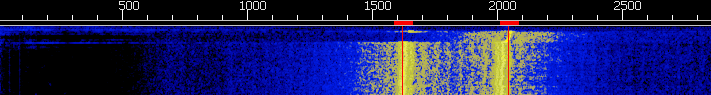
\includegraphics[width=0.9\textwidth]{images/rtty.png}
  \end{center}
  \caption{Spectrogram of a RTTY Transmission (300 baud, 425Hz shift)}
  \label{fig:rtty}
\end{figure}
RTTY, or radio-teletype, is a simple form of frequency shift keying (FSK). Two frequencies are used, representing either a logical `1' or a `0'. Stop and start bits are used to signify the start and end of a transmitter byte. By default no error correction is used, but could be added by the user.

Baud rates for this mode range from 45 up to 300 baud, with higher rates possible. The shift between the two frequencies can be set arbitrarily, but a shift equal to the baud rate or higher (in Hz) is recommended.

RTTY's bandwidth usage can vary depending on the frequency shift and baud rate in use. For example, a 300 baud transmission with a 425Hz shift uses approximately 1KHz of bandwidth. 

RTTY is not very noise resistant - a high SNR is required for correct decoding. It is recommended that some form of checksum be used in the transmission to check received data.

\subsubsection*{DominoEX}
\begin{figure}[h]
  \begin{center}
    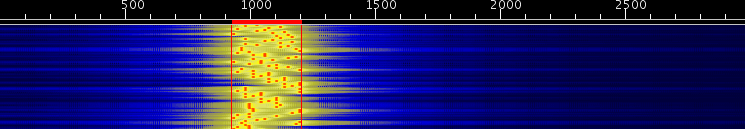
\includegraphics[width=0.9\textwidth]{images/dominoex.png}
  \end{center}
  \caption{Spectrogram of a DominoEX Transmission (7.8125 baud, 346Hz bandwidth)}
  \label{fig:dominoex}
\end{figure}
DominoEX is a MFSK (Multiple Frequency Shift Keying) data mode, developed by Murray Greenman\citep{ref:dominoex}. It uses 18 tones with incremental frequency shift keying, where the data is communicated by the difference between tones, not the tone itself.

A number of variations on DominoEX are available, with baud rates ranging from 4Hz up to 29Hz. User data throughput ranges from 3 to 16 characters per second, and bandwidth requirements range from 173 to 524Hz, depending on the mode used. 

DominoEX is more noise resistant than RTTY, but has very strict timing requirements. Small differences in tone timing, such as if an interrupt is called between tone changes, can cause the decoding software to become confused and stop decoding. This issue was solved by disabling interrupts during transmission. Another solution would be to make the transmission code interrupt based, but this was not implemented.

\section{Prototype System}
To enable proper testing of the transmitter system, a prototype was constructed. The XPlain development board and the AD9835 signal generator were connected together using vero-board, with on-board 3.3V and 5V regulators to allow running everything from a 12V supply. Initially, the regulators were standard linear regulators, but switch-mode regulators were eventually purchased. These switch-mode regulators operate at approximately 80\% efficiency.

\begin{figure}[h]
  \begin{center}
    \includegraphics[width=0.9\textwidth]{images/MainBoard.pdf}
  \end{center}
  \caption{Prototype Mainboard}
  \label{fig:mainboard}
\end{figure}

Figure \ref{fig:mainboard} shows the prototype main-board. This board was connected to the amplifiers via short lengths of coaxial cable, as can be seen in Figure \ref{fig:prototype}. This figure also shows a 1:1 balun, used for matching the $50\Omega$ output to a half-wave dipole antenna (not connected in this image). Other inputs were added to the main-board, for use in the example application (see Section \ref{example_app}).

\begin{figure}[h]
  \begin{center}
    \includegraphics[width=0.9\textwidth]{images/prototype.pdf}
  \end{center}
  \caption{Assembled Prototype System}
  \label{fig:prototype}
\end{figure}

As the Class E amplifier was constructed very late in the project, it has only been tested into a $50\Omega$ dummy load. The 40mW pre-amp however, was tested using a half-wave dipole set-up in the authors backyard. Unfortunately, this could only be received locally around Adelaide, SA, due to the low power.

\begin{table}[h]
\begin{center}
\caption{Main-Board Power Analysis}
\begin{tabular}{l|l|l}
XPlain Board & 100mA @ 3.3v & 330mW\\
AD9835 & 40mA @ 5V & 200mW\\
GPS Module & 120mA @ 3.3V & 396mW\\
5V Regulator Quiescent Current & 16mA @ 12V & 192mW\\
\hline
\textbf{Total} & & 1118mW\\
\end{tabular}
\end{center}
\label{table:mainboard_power}
\end{table}

Current draw of the board was much higher than expected, drawing 155mA @ 12V, or 1.86 Watts. Current draw of various devices of the board were measured, with the results in Table \ref{table:mainboard_power}. We can see that about 740mW of power is unaccounted for. 
Since the XPlain's current draw was measured with it disconnected from the main-board, it's possible some extra power is used to drive the level converters on the board. Some of this power can probably be accounted for in the 5V to 3.3V regulator. Unfortunately, due to the vero-board construction, the rest of the unaccounted power could not be tracked down.


\section{Example Application - High Altitude Balloon Payload}
\label{example_app}
Mid-2010, the author became involved with a local high altitude ballooning group - Project Horus. The Project Horus group use telemetry on the 433MHz ISM band to transmit positioning and temperature data from their payloads, and were interested in other telemetry systems. Terry Baume, the founder of Project Horus, offered to fly a HF telemetry transmitter as a payload on a future launch. This would allow testing of the prototype in the harsh environments present at high altitudes. 

To be able to fly the prototype as a payload a few additions had to be made. First was a way of getting the payload's position - a GPS module. The author already had a GPS module from another project, so this was wired into the main-board. To be able to collect information on the temperatures the payload would experience, Maxim DS18B20 temperature sensors were added. The supply voltage was also fed into one of the ADC inputs via a voltage divider, so it can be measured. To save time, libraries to parse GPS input, and read from the temperature sensors, were ported from the Arduino Project (see Appendix \ref{arduino}).

Data is collected from the inputs every few seconds, and compiled into a single line, containing information as follows:
\texttt{\$\$CALLSIGN,Transmit Count, UTC Time, Latitude, Longitude, Altitude, Speed, Number of GPS Satellites in use, Internal Temperature, External Temperature, Supply Voltage * CRC16 Checksum}\\
This data is then transmitted at 7.037MHz using 300 baud RTTY, with a 425Hz carrier shift.
Below is an example of a generated data sentence:
\begin{verbatim}
$$DARKSIDE,4573,07:04:04,-35.35509,138.44395,32117,98,15,6,-3,10.7*A0F0
\end{verbatim}

This format was chosen as it is mostly compliant with the UK High Altitude Society telemetry protocol\citep{ref:ukhas}. This allows the use of the `dl-fldigi' client to decode, parse, and upload the data to an online system that allows live tracking of high altitude balloons.

\begin{figure}[h]
  \begin{center}
  \begin{tabular}{cc}
    \includegraphics[width=0.685\textwidth]{images/payload_inside.jpg} &
    \includegraphics[width=0.315\textwidth]{images/payload_balloon.jpg}\\
  \end{tabular}
  \end{center}
  \caption{Prototype mounted inside payload box, and view of payload below balloon}
  \label{fig:payload_inside}
\end{figure}

The main-board and pre-amp were mounted inside a polystyrene box, along with a battery pack containing 8 1.5v Energizer Lithium cells. Only the 40mW pre-amp was used, as the power amplifier was not finished yet. A small 1:1 balun was mounted to the side of the pre-amplifier, connected to a half-wave dipole extending outside of the box. An image of the constructed payload, and an image of the payload suspended below a balloon, appear in Figure \ref{fig:payload_inside}.

On the 9th of October 2010 the payload was launched as Horus 8, together with another payload containing the standard UHF telemetry system and a HD video camera. A full write-up appears in Appendix \ref{horus8}. 

The balloon and payloads rose to 32km altitude, and were successfully received all around the state. The HF payload's data was received and decoded as far away as Whyalla, in South Australia's central north, at a distance of approximately 270km.

Throughout the test, the external temperature dropped to $-40^\circ$C. The switch-mode power supplies had not arrived in time for the test, and in-efficient linear regulators had to be used instead. The temperature on the regulators heat-sink was measured to be $75^\circ$C, and this resulted in the payload's internal temperature only dropping to $-5^\circ$C. 

The balloons burst, and after a short chase the payloads ended up landing about 200m offshore, at Carrickalinga (-35.4148, 138.3231), a small beach-side down near Myponga. The payloads were successfully recovered, with only a small amount of salt-water corrosion. The HF payload survived the corrosion, and after some cleaning, works perfectly.


\section{Project Review}
This section looks at how various aspects of the project compared to what was set out in the Design Document\citep{ref:designdoc}. Apart from the project reports, the project's main deliverable was a working prototype, which was successfully designed and built.

\subsection{Project Timeline}
The project timeline, as specified in the Design Document, proved to be very optimistic in practice. Still, a working prototype was finished by Week 3 of Semester 2, albeit with low output power.

\subsection{Project Requirements}
The project's Design Document gave a list of requirements for the project to be considered successful. These are outlined below with corresponding discussions on how the requirements were met, or how the project can be modified to meet them.

\subsubsection{Cold Temperature Operation}
While the whole prototype was not tested, the key components of the design were shown to operate at extremely cold temperatures. In general, the problem was found to be more about controlling temperature \textit{rate of change} rather than controlling temperature itself. Use of foam insulation in the balloon payload successfully prevented fast temperature drops, even with extreme ($-40^\circ$C) external temperatures.

\subsubsection{Data Rate}
While the rate specified in the Design Document (600 baud) is achievable with the prototype hardware, testing was only conducted up to 300 baud. This was a limitation of the data decoding software in use, and could only be overcome by designing and constructing a receiver, which was out of scope for this project.

\subsubsection{Output Power}
The Design Document called for 1W output power, which has almost been achieved (880mW) with the in-development Class E amplifier, albeit at a low efficiency. Further work on the Class E amplifier will raise both the output power, and efficiency.

At the time this report was written, sky-wave propagation had not yet been tested. Calculations from the Design Document suggest the 1W output from the Class E amplifier will be sufficient for reception about 300km away, though this will depend on ionospheric conditions.

\subsubsection{High Efficiency}
While the amplifiers still need work to raise the efficiency, the micro-controller and signal generator operate at a reasonably low power. Power consumption can be reduced even more by increasing the time between transmissions, and cutting power to the RF stage of the circuit when not in use. 

\subsection{Risk Management}
Four major risks were mentioned in the Design Document, and all had to be dealt with during the project.
\subsubsection{Data Loss}
Data loss was listed in the design document as a risk that could cause serious setbacks to the project. Throughout the year, two hard-drive crashes on the authors laptop occurred, requiring restoration from backups. All of the project work was stored on external version control servers, so project work was able to be continued on University machines.

\subsubsection{Construction Delays}
Construction of the AD9834 breakout board was delayed slightly, in most part due to a design error. Shipping delays caused late arrival of some parts required for the flight-test prototype. This resulted in having to use alternative devices, such as linear regulators instead of switch-mode supplies. 

\subsubsection{Dry Ice}
Dry Ice was used for all the cold temperature testing. A workshop risk assessment form had to be completed before experimentation could take place. Use of correct protective equipment prevented any injuries from occurring.

\subsubsection{RF Burns \& Electric Shock}
Since most of the project operated at low voltages, the risk of electric shock was low, and no issues were encountered. The final Class E amplifier stage produced a 40Vp-p output at the drain of the main FET, which had the potential to cause RF burns. Care was taken when working on the amplifier, and no injuries occurred.

\subsection{Project Budget}
\begin{table}[h]
\begin{center}
\caption{Equipment \& Component Purchases}
\begin{tabular}{l|r}
\hline
\textbf{Item} & \textbf{Cost (\$)}\\
\hline
ATXMega100 Breakout Board & 30.80\\
Atmel XPlain Dev Board & 60.58\\
AD9834 DDS IC $\times$ 2 & 26.30\\
TSSOP-20 to Pin Header Breakout Board & 13.70\\
Dry Ice & 10\\
AD8008 $\times$ 2 & 12.20\\
IRF510 $\times$ 5 & 6.15\\
2N4427 $\times$ 2 & 5.96\\
\hline
\textbf{Total} & \textbf{\$165.70}\\
\end{tabular}
\end{center}
\label{proj_costs}
\end{table}
Costs for the project fell well short of the \$250 budget, only totalling \$165.70. Money was saved by using components from the department store, as well as using in-house circuit board manufacturing. The author supplied some items for the project, such as the AVR programmer, the AD9835 breakout board, and the GPS module used in the balloon test. A listing of purchased equipment appears in Table \ref{proj_costs}.

\subsection{Management}
As only one student was working on this project, many of the management processes normally used in group projects were not applicable. However, weekly meetings with the project supervisor ensured the project stayed on track. During a period that the supervisor was away, regular communication via e-mail was used. Problems of a technical nature were mostly handled by a PhD student, Heath Yardley.

\section{Conclusion}
This project produced a working HF telemetry system, providing a hardware and software framework suitable for many different telemetry applications. Testing has shown the hardware in use can operate at extremely low temperatures, as would be experienced in the Antarctic.

The system provides a low-cost data-retrieval solution for remote experiments, and should prove useful to many research efforts.


\newpage
\section*{Glossary}
\begin{description}
\item[Arduino:] A simple embedded systems prototyping platform, using an Atmel ATMega micro-controller.
\item[FSK:] Frequency Shift Keying.
\item[HF:] The `High Frequency' radio band, between 3 \& 30MHz.
\item[PSK:] Phase Shift Keying.
\item[QRSS:] Very slow speed morse code.
\item[XMega:] A 8-bit micro-controller, produced by Atmel.
\end{description}

\section*{References}
\renewcommand*{\refname}{\vspace*{-12mm}}
\begin{thebibliography}{99}
\bibitem{ref:iridium}
Iridium Communications Inc. ``Iridium Satellite Call Plans"" \url{http://www.iridiumphones.com.au/Call\%20Plan\%20Brochure\%20-\%20Post-paid.pdf}, 2010

\bibitem{ref:bomtx}
ACMA Register of Radio-communications Licenses, Met Bureau Site near Corkscrew Rd Montacute \url{http://web.acma.gov.au/pls/radcom/assignment\_search.lookup?pACCESS\_ID=1320447&pDEVICE\_ID=1316356}

\bibitem{ref:bom}
Australian Bureau of Meteorology, ``IPS Online HF Network Frequency Selection Tool" \url{http://www.ips.gov.au/HF\_Systems/7/1/10} , 2010 %[Mar. 14, 2010]

\bibitem{ref:xmega}
Atmel Corporation, ``ATMega128A1 Datasheet'' \url{http://www.atmel.com/dyn/resources/prod_documents/doc8067.pdf}

\bibitem{ref:lpf}
Alexandru Csete, ``Sparrow Overvew'' \url{http://www.oz9aec.net/index.php/all-radios/47-sparrow-40/183-sparrow-overview}

\bibitem{ref:gcode}
Mark Jessop, ``XMega-QRP - Google Code Project'' \url{http://code.google.com/p/xmega-qrp/source/browse/#svn/trunk/XMega_Code}

\bibitem{ref:fldigi}
David Freese, ``FLDigi - A free \& light digital modem program'' \url{http://www.w1hkj.com/Fldigi.html}

\bibitem{ref:dominoex}
Murray Greenman, ``DominoEX - an IFK Mode for HF'' 
\url{http://www.qsl.net/zl1bpu/MFSK/DEX.htm}

\bibitem{ref:ukhas}
UKHAS ``Communications Protocol''
\url{http://ukhas.org.uk/communication:protocol}

\bibitem{ref:dlfldigi}
James Coxon, ``dl-fldigi - Fldigi adapted for use with high altitude balloon tracking'' \url{http://code.google.com/p/dl-fldigi/}

\bibitem{ref:designdoc}
Mark Jessop, ``A Radio Relay System for Remote Sensors in the Antarctic - Design Document'', 2010

\end{thebibliography}

\newpage
\begin{appendices}
\section{XMega Dry Ice Testing}
\label{xmegadryice}
To test the AT-XMEGA128A1 breakout board, the chip was programmed to output the internal clock signal on a I/O pin, and one of the UARTs was programmed to continually send out ``Hello World" at 9600 baud. A LED was also attached to the board, and the chip programmed to flash it at 1Hz. The breakout board assembly was wrapped in bubble wrap (for insulation) with a ribbon cable exiting the insulation to carry the data lines. The insulated board was then placed in a small foam Eski containing approximately 3KG of dry ice. Over the course of an hour, the chip cooled down to -49$^\circ$C, where it stayed for approximately 20 minutes. After shuffling the dry ice slightly, the chip cooled down a further 5$^\circ$C, to -54$^\circ$C at which point the test was aborted. Throughout the test the clock frequency and chip temperature were measured, to produce the plot in Figure \ref{32mhzrc}.


\begin{figure}[h!]
\begin{center}
\includegraphics[width=13cm]{images/32MHzRC.pdf}
\caption{AT-XMEGA128A1 RC Clock Drift}
\label{32mhzrc}
\end{center}
\end{figure}

\begin{figure}[h!]
\begin{center}
\includegraphics[width=13cm]{images/xmega_4.jpg}
\caption{AT-XMEGA128A1 Breakout Board Wrapped in Insulation}
\label{xmega_4}
\end{center}
\end{figure}

\newpage
\begin{figure}[h!]
\begin{center}
\includegraphics[width=13cm]{images/xmega_2.jpg}
\caption{AT-XMEGA128A1 Breakout Board Warming up after testing.}
\label{xmega_2}
\end{center}
\end{figure}

\begin{figure}[h!]
\begin{center}
\includegraphics[width=11cm]{images/xmega_3.jpg}
\caption{Ice forming on the XMEGA's pin headers after testing.}
\label{xmega_3}
\end{center}
\end{figure}

\newpage
\section{Software}
All code for this project has been released under the GPLv3 license, and is available on a Google Code SVN repository. The URL is:
\url{http://code.google.com/p/xmega-qrp/source/browse/#svn/trunk/XMega_Code} 

\subsection{The Arduino Project and the XMega}
\label{arduino}
The Arduino is an open-source electronics prototyping platform based on flexible, easy-to-use hardware and software.
Since many users of the Arduino haven't had much experience in programming, many libraries have been created to fulfil various needs. It's fairly common to begin working on a bit of code to drive some chip, to find that someone has already written a library a few months previously. To quickly get sections of the XMega's codebase working, it was decided to port certain Arduino libraries to the XMega platform. 

Arduino's IDE uses the `wiring' programming language. Wiring is a `C-like' language, following most of C's syntax, to the point that the Arduino IDE uses a collection of C++ libraries to `convert' wiring to C++ for compilation. While these libraries could be ported to the XMega allowing usage of the Arduino IDE for this project, this would have required a lot of work and been out of scope. Instead, the Arduino libraries which were needed (OneWire, DallasTemperature, TinyGPS) were individually ported. This involved replacing various Arduino-specific function calls with generic AVR-C calls, and some other minor code changes. 

\newpage
\section{Schematics \& PCBs}
\subsection{AD8008 Pre-Amp}
\label{ad8008_preamp}
\begin{figure}[h!]
\begin{center}
\includegraphics[width=12cm]{images/AD8008_Schem.pdf}
\caption{AD8008 Pre-Amp Schematic}
\label{ad8008_schem}
\end{center}
\end{figure}
\begin{figure}[h!]
\begin{center}
\includegraphics[width=12cm]{images/AD8008_PCB.pdf}
\caption{AD8008 Pre-Amp PCB Artwork}
\label{ad8008_PCB}
\end{center}
\end{figure}
\newpage
\subsection{AD9834 Breakout Board}
\label{ad9834_breakout}
\begin{figure}[h!]
\begin{center}
\includegraphics[width=12cm]{images/AD9834_Schem.pdf}
\caption{AD9834 Breakout Board Schematic}
\label{ad9834_schem}
\end{center}
\end{figure}
\begin{figure}[h!]
\begin{center}
\includegraphics[width=12cm]{images/AD9834_PCB.pdf}
\caption{AD9834 Breakout Board PCB Artwork}
\label{ad9834_PCB}
\end{center}
\end{figure}


\newpage
\section{Project Horus Launch 8 Write-up}
\label{horus8}
This text was written by Terry Baume, and has been reproduced, with permission, from the Project Horus website. The full text, with images, may be viewed at \url{http://projecthorus.org/?page_id=1497}

\subsubsection*{Technical Information}

\begin{tabular}{ll}
Launch date & 9/10/2010, 12:30pm\\
Landing date & 9/10/2010, 7:00pm\\
Flight duration	& 6.5 hours\\
Launch site & -35.1018, 138.8248\\
Landing site & -35.4148, 138.3231\\
Distance travelled & 57.3 km\\
Maximum altitude & 32,101 m\\
Average ascent rate & 1.5m/s\\
Impact speed & 6 m/s (22 km/h)\\
Payload weight & 1400g\\
Flight computer &	Nut 1.1 flight computer (UHF), HF telemetry experiment\\
GPS module & Falcom FSA03\\
Radio transmitter & Radiometrix NTX2 25mw\\
Video Camera & GoPro HD Hero 1080p\\
Telemetry & 300 baud RTTY, CRC16 checksum on UHF \& HF\\
Tracking & Ground stations (distributed listener), 3 chase cars, web based tracker\\
\end{tabular}

\subsubsection*{Details}

Horus 8 was a test of a HF telemetry system being developed by a friend of ours - Electrical Engineering student \& high altitude balloon enthusiast Mark, as well as the first trial flight of a GoPro HD Hero high definition video camera. It was also planned to fly Adrian's simplex repeater again, though this had to be cut from the payload at the last minute due to launch preparation issues.

Mark's HF telemetry system was built around an Atmel XMega \& signal generator, as well as an amp he'd built. It was putting out approx 40mW of power on 7.037MHz, transmitting 300b RTTY, including GPS location, temperature \& battery voltages. The goal of the flight was to test the performance of the system in both harsh conditions \& over a long range.

This launch was also a precursor to a launch we'd planned the next day (10/10/10) for the One Day on Earth movement - we were trialling HD video using a GoPro HD Hero. It was hoped that the same payload (minus the HF experiment) would be flown the next day to capture footage for One Day on Earth.

As part of the video launch we were also experimenting with a trailing fin design - intended to keep the payload pointed in one direction in the wind, to avoid the usual spinning - this seemed to work well!



\subsubsection*{Launch}

Launch conditions on the day were great - clear skies, minimal wind at ground level and being the beginning of spring, pleasantly warm. Graham VK5GH had also offered us the use of his garage for setup \& inflation, which was a great help with this more complex payload.

Grant VK5GR was also recording video footage of the whole day, which we'll no doubt see online soon!

Launch preparations went smoothly for the most part, until we attempted to tie the balloon off - unfortunately it slipped out of out gloved hands, and before we could catch it, it was bobbing around the ceiling, with it's open neck quickly pouring out helium!  Fortunately thanks to some quick thinking of behalf of Graham, we managed to retrieve the balloon with a ladder before too much gas was lost, and continue filling. The loss of gas meant that we needed to reduce our payload mass, so the repeater was pulled from the flight (little did we know this would end up to be a fortunate removal!).

The balloon train for this launch was the longest yet - the HF antenna for Mark's payload spanned 10m both above and below it - with the rest of the gear (radar reflector, parachute, etc), we were looking at a very long balloon train!

Our intended ascent rate for this launch was 3m/s - fortunately weather conditions for the day were ideal, with predictions suggesting the balloon would drift some distance away \& then return to almost exactly the launch site, regardless of the ascent rate.

A few minutes before launch our payloads were assembled \& ready to go, with one exception - my UHF telemetry system had not acquired GPS lock, despite having had a good deal of time to do so. After ~20 minutes of waiting, the payload started broadcasting valid coordinates, so we sealed everything up and launched.

\subsubsection*{Flight}

No sooner than we'd launched we realised we had a couple of issues: our ascent rate was far too slow (~1m/s), and the primary telemetry system (UHF) had lost lock. With Mark's system having never been tested over a long range or at altitude, the thought of relying on an untested system was a bit worrying - thankfully it seemed to be performing perfectly!

The ascent rate posed another issue - with the payload only rising at 1m/s, it would be many hours before we reached apogee, which meant the payload would land after dark. Fortunately predictions suggested the landing site would not be moved too far, so we hoped that recovery would still be relatively easy.

About 20 minutes after launch, my telemetry system finally got lock - and held it for the remainder of the flight. Fortunately for us, the ascent rate increased to 1.5-2m/s as the gas inside the balloon warmed as it rose above the clouds - meaning that it looked like the payload would before dark after all - though it would still be a very long flight. The obvious fix for this was to settle down and have a great BBQ \& beer courtesy of Matt, Grant and Scott (thanks guys!).

\subsubsection*{Recovery}

4-5 hours after launch, the balloon had reached ~30km, had turned around \& was heading back towards the launch site at 100km/h. We packed up the cars and set out to the predicted landing site (near Meadows, only a few km away), splitting up and taking different roads along the way.

We soon noticed something rather alarming - rather than bursting, the balloon had reached a state of float at ~32km altitude. It wasn't ascending or descending, but it was still moving along at 100km/h! We frantically tried to stay ahead of it \& get into position to intercept it when it did burst, but this did not prove easy. The balloon shot past the expected landing site and kept on going - heading straight out to sea. For the next hour, our chase cars raced towards the coast, all the while hoping the balloon would burst

Before long, the balloon was above the sea, and our hopes shifted to it bursting and our payload landing on Kangaroo Island - this would have made recovery almost impossible (access is by ferry crossing only), but it was always possible that someone could find the payload \& return it to us via the contact details listed on the payload. However, at the last possible second, the balloon burst! We knew that a lower altitude wind inversion meant it was still possible our payload could end up on land, but it was too close to call - looking back now, if the balloon had burst even a few seconds later (it was heading out to sea at 100km/h), recovery would have been entirely impossible without a boat.

Our 3 chase teams were now scrambling to get to the expected landing site (Carrickalinga, a tiny beachside holiday town) - we all arrived within a few moments of one another, with Adrian \& Matt's chase teams arriving in time to watch the payload come down - into the sea!

The payload landed only 50m or so out to sea - but the open parachute caught the wind and started dragging it out to sea. By the time I'd arrived (only 1-2 minutes later), it was far enough out that it was very hard to spot, though the GPS tracking was still working! There was some scrambling to try to get a kayak spotted down the beach ready to recover the payload, but I decided to go for it before the payload ended up too far out and lost forever.

After a few failed attempts at getting the kayak going (as it turns out Maxtrax do not make good paddles!), Joel managed to get hold of an actual paddle from a local \& came out to help me bring the payload back in - the current and wind heading out to sea was making pulling the balloon train (complete with parachute) back to shore very hard going.

\subsubsection*{Results/post-mortem}

Once back on dry land, I went off to seek a shower before I froze to death in the wind - thanks to all the locals who helped out, especially for letting a stranger invade their bathroom for a hot shower! 

The rest of the chase teams started pulling apart the payloads and irrigating all the electronics to displace as much sea water as possible - air compressors in 4WD's certainly helped in this regard! Mark's HF payload was quite well sealed and did not suffer a great deal of water ingress - though still enough to cause some corrosion. However, the main payload containing the video did not fare so well - the hole the lens stuck out of allowed water in, which also resulted in the payload being dragged under water on it's way back to shore. The flight computer was very corroded, to the extent that some tracks were entirely eaten away.

\subsubsection*{Conclusion}

Whilst this launch was without a doubt the most challenging so far in terms of recovery \& the only flight on which equipment has been lost/damaged, it was not without success. The HF telemetry experiment went very well, and was logged for the duration of the entire flight. The HF telemetry did prove more difficult to decode while mobile, but was rock solid when stationary.

Furthermore, our stabilising fin design proved to be quite successful, limiting the spin on the payload, and our chase teams gained a good deal of experience in tracking in difficult circumstances. The long flight time also presented an ideal opportunity for systems testing \& setup - this was the first time Matt VK5ZM's tracking systems had been used with the Horus telemetry systems.

Unfortunately the length of the flight \& the water damage sustained meant the payload could not be flown the following day for One Day on Earth - by the time we had recovered everything and were back at the launch site, it was quite late. However, weather predictions for the next day were not favourable, and it seemed likely that we might end up in the water if we launched that day too.

The failures of this launch essentially come down to under-inflation of the balloon - this caused both the low ascent rate and the float situation, very nearly resulting in the loss of the payload. We'll take these failings into account in future launches and somewhat re-think the gas/lift calculations used.

I'd like the give a big thanks to everybody who helped to make the day possible, especially to Grant VK5GR for funding the Helium and Graham VK5GH \& Carol for letting us spend the entire day at their place (and looking after us!). An extra thanks to everybody who helped with tracking - the data relayed by stations via the internet is invaluable to us in the chase cars when surrounding conditions (trees/hills etc) make decoding a radio signal difficult.

With any luck the next launch will go a little more smoothly! 

\end{appendices}

\end{document}